\section{Why two controllers}
\label{sec:why}

\subsection{What ARTIQ is good at, and what it is not}

ARTIQ schedules \emph{events} on a timeline. A kernel running on the Kasli
core device writes RTIO output events (a TTL edge, a DDS register write, a
DAC value) with a timestamp in machine units (1\,mu = 1\nsu\ on this
machine, coarse clock 8\nsu)\footnote{\file{k-exp/kexp/util/db/device\_db.py}
(\code{ref\_period = 1e-9}); \code{t\_rtio = 8e-9} in
\file{kexp/config/expt\_params.py}.}, and the gateware plays them out
deterministically. The kernel CPU (a soft core) does the bookkeeping: it
runs the Python-compiled control flow, submits events into FIFOs ahead of
real time, and blocks on input events (\code{timestamp\_mu}). Two consequences
matter here:

\begin{itemize}[nosep]
  \item Output timing is exact to the coarse clock, \emph{as long as the CPU
    stays ahead}. If an event is submitted after its timestamp has passed, the
    kernel raises \code{RTIOUnderflow}. The lab's scan loop catches it and
    aborts the run (section~\ref{sec:handoff:crash}).
  \item Real-time \emph{computation} is slow. The Bayesian feedback loop of
    section~\ref{sec:feedback} runs a 21-point posterior update on the kernel
    CPU in double precision; the budget reserved for it is
    \code{t\_calculation\_slack\_compensation\_mu} $= 0.7\us\times m + 15\us =
    29.7\us$ for $m = 21$, plus an 18.4\us\ ``fifo'' allowance, so each
    feedback cycle is 57--61\us\ long for 10--14\us\ of physics.\footnote{\file{k-exp/kexp/experiments/HF\_experiments/feedback/expt\_params\_feedback.py},
    lines 79--81; \file{k-exp/kexp/base/feedback.py}, \code{compute\_t\_between\_pulses\_mu}.}
    The reading of the analog integrator through the Sampler is itself a
    blocking SPI transaction that leaves ``slack $\sim$zero'' on return.
\end{itemize}

\subsection{What the OPX+ is good at}

The Quantum Machines OPX+ is a pulse processor: 18 real-time cores, each
owning one \emph{element} (a logical channel bound to analog/digital ports),
running a compiled QUA program in lock-step at a 4\nsu\ clock cycle
(cc).\footnote{\file{k-exp/kexp/control/opx/units.py}: \code{CLOCK\_NS = 4},
\code{MIN\_PULSE\_CC = 4}.} Its strengths, relative to ARTIQ, are:

\begin{itemize}[nosep]
  \item \textbf{Real-time arithmetic next to the pulses.} QUA has 32-bit
    integers and 4.28 fixed-point reals (range $[-8, 8)$, step $2^{-28}$),
    a \code{Math} library (\code{sqrt}, \code{inv}, \code{exp}, \code{cos2pi},
    \code{sin2pi}, whole-array \code{sum}/\code{max}/\code{argmax}/\code{dot}),
    and a \code{measure} statement whose integrated result is usable by the
    next statement. The posterior update becomes a few microseconds of
    fixed-point work interleaved with the pulses, not tens of microseconds of
    soft-CPU floating point.
  \item \textbf{Deterministic timing by construction.} A statement whose
    inputs are known at compile time is scheduled without gaps; a statement
    that depends on a QUA variable adds ``a few cycles''. Either way the
    element clock advances by exactly the durations played and waited, which
    is what section~\ref{sec:feedback} relies on.
  \item \textbf{Sticky elements} (section~\ref{sec:why:sticky}) hold an
    analog level or a digital marker across statements, so a CW tone or a
    switch level is set once and stays.
  \item \textbf{Streams} carry measurement results and timestamps back to the
    host asynchronously, without stalling the program.
\end{itemize}

What the OPX+ does \emph{not} do for us: it has no shutters, no coils, no
camera, no line trigger, no 200-parameter experiment object. The MOT, the
tweezer loading, the shutters, the field, the imaging and every other part of
the shot stay on ARTIQ. The OPX is handed the atoms for one window per shot
(section~\ref{sec:handoff}) and hands them back.

\subsection{The wires}
\label{sec:why:wires}

Figure~\ref{fig:wires} shows every physical connection the integration uses.
There are three logic wires between the two controllers and four beam-path
connections.

\begin{figure}[htbp]
\centering
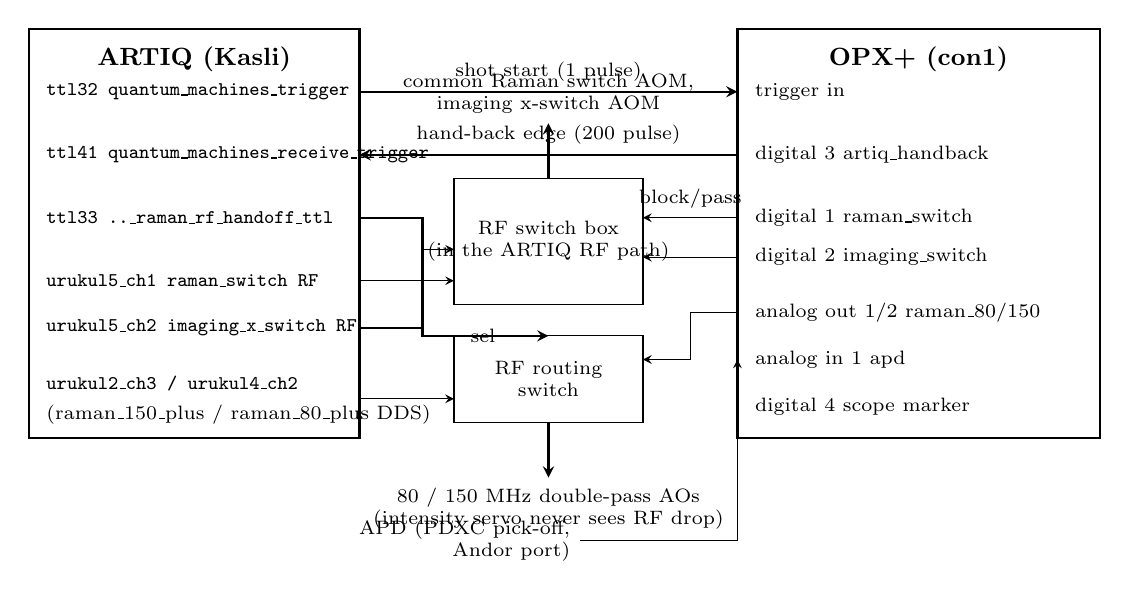
\begin{tikzpicture}[>=stealth, font=\small, x=1cm, y=1cm]
  % ARTIQ box
  \draw[thick] (0,0) rectangle (4.2,5.2);
  \node[anchor=north] at (2.1,5.1) {\textbf{ARTIQ (Kasli)}};
  \node[anchor=west, font=\scriptsize\ttfamily] at (0.1,4.4) {ttl32 quantum\_machines\_trigger};
  \node[anchor=west, font=\scriptsize\ttfamily] at (0.1,3.6) {ttl41 quantum\_machines\_receive\_trigger};
  \node[anchor=west, font=\scriptsize\ttfamily] at (0.1,2.8) {ttl33 ..\_raman\_rf\_handoff\_ttl};
  \node[anchor=west, font=\scriptsize\ttfamily] at (0.1,2.0) {urukul5\_ch1 raman\_switch RF};
  \node[anchor=west, font=\scriptsize\ttfamily] at (0.1,1.4) {urukul5\_ch2 imaging\_x\_switch RF};
  \node[anchor=west, font=\scriptsize\ttfamily] at (0.1,0.7) {urukul2\_ch3 / urukul4\_ch2};
  \node[anchor=west, font=\scriptsize] at (0.1,0.3) {(raman\_150\_plus / raman\_80\_plus DDS)};
  % OPX box
  \draw[thick] (9.0,0) rectangle (13.6,5.2);
  \node[anchor=north] at (11.3,5.1) {\textbf{OPX+ (con1)}};
  \node[anchor=west, font=\scriptsize] at (9.1,4.4) {trigger in};
  \node[anchor=west, font=\scriptsize] at (9.1,3.6) {digital 3 \code{artiq\_handback}};
  \node[anchor=west, font=\scriptsize] at (9.1,2.8) {digital 1 \code{raman\_switch}};
  \node[anchor=west, font=\scriptsize] at (9.1,2.3) {digital 2 \code{imaging\_switch}};
  \node[anchor=west, font=\scriptsize] at (9.1,1.6) {analog out 1/2 \code{raman\_80/150}};
  \node[anchor=west, font=\scriptsize] at (9.1,1.0) {analog in 1 \code{apd}};
  \node[anchor=west, font=\scriptsize] at (9.1,0.4) {digital 4 scope marker};
  % logic wires
  \draw[->, thick] (4.2,4.4) -- (9.0,4.4) node[midway, above, font=\scriptsize] {shot start (1\us\ pulse)};
  \draw[<-, thick] (4.2,3.6) -- (9.0,3.6) node[midway, above, font=\scriptsize] {hand-back edge (200\nsu\ pulse)};
  % RF routing switch
  \draw (5.4,0.2) rectangle (7.8,1.3);
  \node[font=\scriptsize, align=center] at (6.6,0.75) {RF routing\\switch};
  \draw[->, thick] (4.2,2.8) -- (5.0,2.8) -- (5.0,1.3) -- (6.6,1.3) node[pos=0.3, right, font=\scriptsize] {sel};
  \draw[->] (4.2,0.5) -- (5.4,0.5);
  \draw[->] (9.0,1.6) -- (8.4,1.6) -- (8.4,1.0) -- (7.8,1.0);
  \draw[->, thick] (6.6,0.2) -- (6.6,-0.5) node[below, font=\scriptsize, align=center] {80 / 150 MHz double-pass AOs\\(intensity servo never sees RF drop)};
  % RF switch box
  \draw (5.4,1.7) rectangle (7.8,3.3);
  \node[font=\scriptsize, align=center] at (6.6,2.5) {RF switch box\\(in the ARTIQ RF path)};
  \draw[->] (4.2,2.0) -- (5.4,2.0);
  \draw[->] (4.2,1.4) -- (5.0,1.4) -- (5.0,2.4) -- (5.4,2.4);
  \draw[->] (9.0,2.8) -- (7.8,2.8) node[midway, above, font=\scriptsize] {block/pass};
  \draw[->] (9.0,2.3) -- (7.8,2.3);
  \draw[->, thick] (6.6,3.3) -- (6.6,4.0) node[above, font=\scriptsize, align=center] {common Raman switch AOM,\\imaging x-switch AOM};
  % APD
  \draw[->] (7.0,-1.3) -- (9.0,-1.3) -- (9.0,1.0);
  \node[anchor=east, font=\scriptsize, align=right] at (7.0,-1.3) {APD (PDXC pick-off,\\Andor port)};
\end{tikzpicture}
\caption{Every connection the integration uses. Channel names are the
\code{ttl\_frame}/\code{dds\_frame} attributes in
\file{k-exp/kexp/config/ttl\_id.py} (lines 64--66) and
\file{dds\_id.py}; OPX ports are the constants at the top of
\file{k-exp/kexp/control/opx/opx\_config.py}. The RF routing switch and the
RF switch box are the lab's own hardware (2026-09 wiring); the OPX never
sees the AOMs directly except through them.}
\label{fig:wires}
\end{figure}

\paragraph{The three logic wires.}
\begin{enumerate}[nosep]
  \item \code{ttl32} $\to$ OPX trigger input. ARTIQ pulses it for
    \code{T\_OPX\_TRIGGER\_PULSE} $= 1\us$ to start one OPX shot. The OPX
    samples this input at 250\,MHz; QM publishes no trigger-to-output
    latency (milestone M1).\footnote{\file{k-exp/kexp/base/control.py}
    line 34; \file{k-exp/kexp/config/ttl\_id.py} line 65.}
  \item OPX digital 3 (\code{artiq\_handback}) $\to$ \code{ttl41}, a
    \code{TTLInOut} gated for rising edges. The OPX plays a 200\nsu\ pulse
    here when its body is done; ARTIQ's kernel is blocked in
    \code{timestamp\_mu} waiting for it.
  \item \code{ttl33} $\to$ the RF routing switch. High = the 80 and
    150\,MHz double-pass AOs are driven by OPX analog outputs 1 and 2; low =
    by the ARTIQ DDSs \code{raman\_80\_plus}/\code{raman\_150\_plus}.
\end{enumerate}

\paragraph{The beam-path connections.} OPX digital 1 and 2 drive an RF
switch box \emph{in the ARTIQ RF path} of the common Raman switch AOM
(\code{urukul5\_ch1}) and the imaging x-switch AOM (\code{urukul5\_ch2}).
OPX analog 1/2 carry the 80/150\,MHz AO tones during the window. The APD
signal enters OPX analog input 1. Digital 4 is a scope marker played during
every ADC window and does nothing else.

\subsection{The truth table}
\label{sec:why:truth}

\begin{table}[htbp]
\centering
\small
\begin{tabular}{@{}llll@{}}
\toprule
line & level & meaning & who sets it \\
\midrule
OPX digital 1 (\code{raman\_switch}) & HIGH & ARTIQ RF to the Raman switch AOM \textbf{blocked} & OPX op \code{block} \\
 & LOW & RF \textbf{passes} (idle state with no job) & OPX op \code{pass} / no job \\
OPX digital 2 (\code{imaging\_switch}) & HIGH / LOW & same, imaging x-switch AOM & same \\
OPX digital 3 (\code{artiq\_handback}) & rising edge & ``body done, take the beams back'' & OPX op \code{trigger} \\
ARTIQ \code{ttl33} & HIGH & 80/150 AOs driven by OPX analog 1/2 & kernel \\
 & LOW & 80/150 AOs driven by ARTIQ DDSs & kernel, idle \\
ARTIQ \code{urukul5\_ch1/2} switch & ON & steady-state RF offered to the switch box & kernel, only inside the window \\
\bottomrule
\end{tabular}
\caption{Polarity of every line, from the truth table in
\file{k-exp/kexp/control/opx/opx\_config.py} (module docstring and
\code{BLOCK\_LEVEL = 1}). ``Block'' is the high level on purpose: with no
job running the OPX lines idle low, so ARTIQ gates its own light in every
non-OPX run exactly as before.}
\label{tab:truth}
\end{table}

The consequence that shapes the whole handshake: \emph{during an OPX window
ARTIQ turns its switch-AOM RF on steady-state and leaves it on}; the OPX then
makes light by opening (\code{pass}) and closing (\code{block}) the switch
box. An exposure of duration $d$ is literally \code{play('pass', 'raman\_switch',
duration=d)} followed immediately by \code{play('block', 'raman\_switch')}.
Because the switch element is sticky-digital, the line stays low for exactly
$d$ and there is no gap before the re-block.\footnote{\file{k-exp/kexp/control/opx/context.py},
\code{OPXShotContext.\_expose}.}

\subsection{Sticky elements}
\label{sec:why:sticky}

A QUA element declared \code{'sticky': \{'analog': True, 'digital': True,
'duration': ...\}} holds the last analog sample and the last digital marker
level after a pulse ends, until the next pulse on that element overrides it.
Three facts about sticky behaviour drive our design (all from QM's feature
guide, verified offline only):

\begin{enumerate}[nosep]
  \item \textbf{Analog sticky plays \emph{add} to the held value.} Playing a
    latch pulse twice doubles the amplitude. The customer script
    \file{00g\_hello\_atoms\_apd.py} looped three times without a
    \code{ramp\_to\_zero} and would have driven \code{raman\_B} from 0.325\,V to
    0.650\,V on shot 2 (beyond the $\pm 0.5$\,V full scale). This is why the
    builder latches the analog drives \textbf{once per run}, in the program
    prologue, and ramps them to zero once in the epilogue
    (section~\ref{sec:program:skeleton}).
  \item \textbf{Digital sticky needs \code{analog: True}.} The QOP rejects a
    job whose element is digital-sticky but not analog-sticky (``sticky
    digital but analog sticky wasn't set'', seen 2026-09-23). Our switch
    elements have no analog port at all and set \code{analog: True} anyway;
    QM's own template instead gave each gate a dummy analog port. Whether
    the QOP accepts a port-less sticky element is an M1 item.
  \item \textbf{A sticky element ramps back to its DC offset at the end of
    the program}, i.e.\ when the job is halted the lines return to idle (low =
    pass). What the digital lines do on \code{job.halt()} \emph{mid-block} is
    not documented -- M1.
\end{enumerate}

\subsection{Why the analog drives are latched and the switch AOM is gated}

The two Raman beams reach the atoms through the 80 and 150\,MHz double-pass
AOs (one per beam, setting the two-photon frequency) and a \emph{common}
switch AOM (setting the pulse envelope). The double-pass AOs sit inside an
intensity servo that must never see its RF drop; the switch AOM's thermal
load depends on its duty cycle. Hence:

\begin{itemize}[nosep]
  \item The OPX \emph{drives} the 80/150 AOs with sticky CW tones latched
    once per run, at exactly the frequencies \code{prep\_raman()} would have
    programmed on the ARTIQ DDSs (the same \code{RamanBeamPair.ao\_frequencies}
    split, section~\ref{sec:program:config}). The routing switch
    (\code{ttl33}) decides whose tone reaches the AOs; the tone itself never
    stops during the run.
  \item The OPX \emph{gates} the switch AOM by blocking/passing ARTIQ's own
    steady-state RF. The OPX does not synthesise the switch RF and does not
    control its amplitude.
\end{itemize}

\paragraph{Why \code{prep\_raman()} stays.} Before the handoff, ARTIQ still
runs \code{prep\_raman()}: it initialises the \code{RamanBeamPair}, plays a
3\,ms warm-up pulse on the switch AOM \emph{with the shutter still closed},
waits 10\us, opens the Raman shutter (3\,ms), waits for the 60\,Hz line
trigger and adds 4.7\,ms.\footnote{\file{k-exp/kexp/base/control.py},
\code{prep\_raman}, lines 154--182.} The warm-up thermally loads the very
AOM the OPX will gate; the OPX's sticky drives keep only the 80/150 AOs
warm and are no substitute. The shutter and the line-trigger phasing are
ARTIQ hardware the OPX cannot touch. This is decision D8 of the spec and is
10.7--28.2\,ms per shot -- by far the largest fixed cost in an OPX shot, and
not handshake waste.
